% ============================================================
%  CS3401 – Chapter 3: Brute Force & Exhaustive Search
% ============================================================
\documentclass[aspectratio=169]{beamer}
% ============================================================
%  CS3401 – Algorithm Design and Analysis
%  Shared Beamer Theme (input this file in every chapter)
%  Prince Sattam Bin Abdulaziz University – CCES
% ============================================================

% ---------- PACKAGES ----------------------------------------
\usepackage[utf8]{inputenc}
\usepackage[T1]{fontenc}
\usepackage{lmodern}
\usepackage{amsmath,amssymb,amsthm}
\usepackage{tikz}
\usepackage{pgfplots}
\usepackage{booktabs}
\usepackage{xcolor}
\usepackage{graphicx}
\usepackage{listings}
\usepackage[normalem]{ulem}
\usepackage{algorithm}
\usepackage{algpseudocode}
\usepackage{multicol}
\usepackage{array}
\usepackage{colortbl}
\usepackage{tabularx}
\usepackage{makecell}

\usetikzlibrary{
  arrows.meta, shapes.geometric, shapes.symbols,
  positioning, calc, fit, backgrounds,
  decorations.pathreplacing, decorations.markings,
  matrix, chains, trees
}
\pgfplotsset{compat=1.18}

% ---------- COLOR PALETTE -----------------------------------
\definecolor{PrimaryDark}{RGB}{10,72,92}
\definecolor{PrimaryMid}{RGB}{18,114,145}
\definecolor{PrimaryLight}{RGB}{185,224,238}
\definecolor{AccentOrange}{RGB}{210,103,22}
\definecolor{AccentYellow}{RGB}{252,198,40}
\definecolor{SuccessGreen}{RGB}{32,122,66}
\definecolor{AlertRed}{RGB}{172,46,46}
\definecolor{CodeBg}{RGB}{244,246,250}
\definecolor{DarkText}{RGB}{28,32,40}
\definecolor{LightRule}{RGB}{210,225,232}
\tikzset{processstep/.style={draw=PrimaryMid, fill=PrimaryLight!35, rounded corners=2pt,
  align=center, minimum width=4.2cm, minimum height=0.55cm, font=\small}}

% ---------- BEAMER SETTINGS ---------------------------------
\setbeamertemplate{navigation symbols}{}
\setbeamertemplate{caption}[numbered]

% Fonts
\setbeamerfont{normal text}{size=\small}
\setbeamerfont{title}{series=\bfseries,size=\LARGE}
\setbeamerfont{subtitle}{series=\normalfont,size=\large}
\setbeamerfont{frametitle}{series=\bfseries,size=\large}
\setbeamerfont{framesubtitle}{series=\normalfont,size=\small}
\setbeamerfont{block title}{series=\bfseries,size=\normalsize}
\setbeamerfont{footline}{size=\tiny}
\addtobeamertemplate{frame begin}{\small\enlargethispage{1cm}}{}
\setlength{\tabcolsep}{2pt}

% Colors
\setbeamercolor{normal text}{fg=DarkText,bg=white}
\setbeamercolor{frametitle}{bg=PrimaryDark,fg=white}
\setbeamercolor{title}{fg=white}
\setbeamercolor{subtitle}{fg=PrimaryLight}
\setbeamercolor{author}{fg=white}
\setbeamercolor{date}{fg=PrimaryLight}
\setbeamercolor{institute}{fg=PrimaryLight}
\setbeamercolor{block title}{bg=PrimaryMid,fg=white}
\setbeamercolor{block body}{bg=PrimaryLight!35,fg=DarkText}
\setbeamercolor{block title alerted}{bg=AlertRed,fg=white}
\setbeamercolor{block body alerted}{bg=AlertRed!12,fg=DarkText}
\setbeamercolor{block title example}{bg=SuccessGreen,fg=white}
\setbeamercolor{block body example}{bg=SuccessGreen!12,fg=DarkText}
\setbeamercolor{itemize item}{fg=PrimaryMid}
\setbeamercolor{itemize subitem}{fg=AccentOrange}
\setbeamercolor{enumerate item}{fg=PrimaryMid}
\setbeamercolor{enumerate subitem}{fg=AccentOrange}
\setbeamercolor{alerted text}{fg=AlertRed}
\setbeamercolor{structure}{fg=PrimaryMid}
\setbeamercolor{section in toc}{fg=PrimaryDark}
\setbeamercolor{section in toc shaded}{fg=PrimaryDark}
% override Beamer's transparency-based shading so TOC entries stay fully visible
\setbeamertemplate{section in toc shaded}{\inserttocsection\par}
\setbeamercolor{subsection in toc}{fg=PrimaryMid}
\setbeamercolor{footer rule}{bg=LightRule}

% Item symbols
\setbeamertemplate{itemize item}{%
  \scriptsize\raise1.5pt\hbox{\color{PrimaryMid}$\blacktriangleright$}}
\setbeamertemplate{itemize subitem}{%
  \scriptsize\raise1pt\hbox{\color{AccentOrange}$\bullet$}}
\setbeamertemplate{itemize subsubitem}{%
  \scriptsize\raise1pt\hbox{\color{PrimaryDark}$\circ$}}
\setbeamertemplate{enumerate item}{%
  \color{PrimaryMid}\textbf{\insertenumlabel.}}

% Frame title
\makeatletter
\setbeamertemplate{frametitle}{%
  \nointerlineskip
  \begin{beamercolorbox}[wd=\paperwidth,ht=2.4em,dp=0.9em,%
                         leftskip=1.2em,rightskip=1.2em]{frametitle}
    \usebeamerfont{frametitle}\insertframetitle\strut
    \ifx\insertframesubtitle\@empty\else
      \hspace{0.6em}\textcolor{PrimaryLight!80}{\footnotesize|}\hspace{0.4em}%
      {\usebeamerfont{framesubtitle}\textcolor{PrimaryLight}\insertframesubtitle}%
    \fi
  \end{beamercolorbox}
  \nointerlineskip
  \begin{beamercolorbox}[wd=\paperwidth,ht=0.3pt,dp=0pt]{structure}
  \end{beamercolorbox}
}
\makeatother

% Footer
\setbeamertemplate{footline}{%
  \begin{beamercolorbox}[wd=\paperwidth,ht=0.4pt,dp=0pt]{footer rule}{}
  \end{beamercolorbox}
  \leavevmode
  \hbox{%
    \begin{beamercolorbox}[wd=0.60\paperwidth,ht=1.8em,dp=0.6em,leftskip=1em]{normal text}%
      \textcolor{PrimaryDark}{\tiny\textbf{CS3401} \textendash{} Algorithm Design \& Analysis%
        \quad\textbar\quad CCES, PSAU}%
    \end{beamercolorbox}%
    \begin{beamercolorbox}[wd=0.40\paperwidth,ht=1.8em,dp=0.6em,rightskip=1em,right]{normal text}%
      \textcolor{PrimaryDark}{\tiny\insertshorttitle%
        \quad\textbar\quad\insertframenumber\,/\,\inserttotalframenumber}%
    \end{beamercolorbox}%
  }%
}

% Title page
\setbeamertemplate{title page}{%
  
\begin{tikzpicture}[remember picture,overlay]
    \fill[PrimaryDark](current page.north west) rectangle (current page.south east);
    \fill[PrimaryMid,opacity=0.45]
      ([shift={(2.5cm,-2.5cm)}]current page.north east) circle(5.5cm);
    \fill[AccentOrange,opacity=0.10]
      ([shift={(-1.5cm,2.0cm)}]current page.south west) circle(4.2cm);
    \draw[white,opacity=0.08,line width=40pt]
      ([shift={(0cm,-0.5cm)}]current page.north west)
      to[out=-30,in=210]
      ([shift={(0cm,0.5cm)}]current page.south east);
  \end{tikzpicture}%
  \vspace{0.7cm}
  \begin{center}
    {\tiny\textcolor{PrimaryLight}{\textbf{CCES} \textendash{}
      College of Computer Engineering and Sciences}}\\[0.2em]
    {\tiny\textcolor{PrimaryLight}{Prince Sattam Bin Abdulaziz University}}\\[1.2em]
    {\footnotesize\textcolor{AccentYellow}{\textbf{CS3401 \textendash{} Algorithm Design and Analysis}}}\\[1.5em]
    \textcolor{PrimaryMid}{\rule{0.55\textwidth}{0.6pt}}\\[0.9em]
    {\Large\usebeamerfont{title}\textcolor{white}{\inserttitle}}\\[0.4em]
    {\small\usebeamerfont{subtitle}\textcolor{PrimaryLight}{\insertsubtitle}}\\[0.7em]
    \textcolor{PrimaryMid}{\rule{0.55\textwidth}{0.6pt}}\\[1.2em]
    {\footnotesize\textcolor{PrimaryLight}{\insertdate}}\\[0.6em]
    % Instructors row
    \begin{tikzpicture}[baseline=(current bounding box.center)]
      % Dr. Khalil – rounded photo
      \begin{scope}
        \clip (-3.2,0) circle (0.58cm);
        \node at (-3.2,0)
          {
\includegraphics[width=1.16cm,height=1.16cm,keepaspectratio=false]{khalil}};
      \end{scope}
      \draw[white,line width=0.9pt] (-3.2,0) circle (0.58cm);
      \node[text=white,font=\scriptsize\bfseries,anchor=west] at (-2.54,0)
        {Dr.\ Khalil Chebil};
      % Dr. Esraa – placeholder circle
      \draw[white,line width=0.9pt] (1.2,0) circle (0.58cm);
      \node[text=PrimaryLight,font=\normalsize\bfseries] at (1.2,0) {E};
      \node[text=white,font=\scriptsize\bfseries,anchor=west] at (1.86,0)
        {Dr.\ Esraa};
    \end{tikzpicture}
  \end{center}%
}

% Auto section-divider slide — background set via Beamer color system for reliability
\AtBeginSection[]{%
  {%
    \setbeamercolor{background canvas}{bg=PrimaryDark}%
    \begin{frame}[plain,noframenumbering]
      \begin{tikzpicture}[remember picture,overlay]
        \fill[PrimaryMid,opacity=0.35]
          ([shift={(0cm,-1.5cm)}]current page.north) circle(6.5cm);
        \node[text=white,opacity=0.06,font=\fontsize{120}{120}\bfseries]
          at ([shift={(-1cm,0cm)}]current page.center)
          {\insertsectionnumber};
      \end{tikzpicture}
      \vfill
      \begin{center}
        {\large\textcolor{AccentYellow}{\textbf{Section \insertsectionnumber}}}\\[0.6em]
        {\LARGE\textcolor{white}{\textbf{\insertsectionhead}}}
      \end{center}
      \vfill
    \end{frame}
  }%
}

% ---------- LISTINGS STYLE ----------------------------------
\lstset{
  basicstyle=\ttfamily\footnotesize,
  backgroundcolor=\color{CodeBg},
  keywordstyle=\color{PrimaryMid}\bfseries,
  commentstyle=\color{SuccessGreen}\itshape,
  stringstyle=\color{AccentOrange},
  numberstyle=\tiny\color{gray!70},
  frame=tb,
  framerule=0.5pt,
  rulecolor=\color{PrimaryLight},
  numbers=left,
  numbersep=6pt,
  showstringspaces=false,
  breaklines=true,
  tabsize=2,
  xleftmargin=1.8em,
  framexleftmargin=1.8em,
  captionpos=b,
  language=Java,
  morekeywords={var,let,const}
}

% ---------- PSEUDOCODE STYLE --------------------------------
\algrenewcommand\algorithmicprocedure{\textbf{Algorithm}}
\algrenewcommand\algorithmicfunction{\textbf{Function}}
\algrenewcommand\algorithmicif{\textbf{if}}
\algrenewcommand\algorithmicelse{\textbf{else}}
\algrenewcommand\algorithmicthen{\textbf{then}}
\algrenewcommand\algorithmicwhile{\textbf{while}}
\algrenewcommand\algorithmicfor{\textbf{for}}
\algrenewcommand\algorithmicforall{\textbf{for all}}
\algrenewcommand\algorithmicreturn{\textbf{return}}
\algrenewcommand\algorithmicend{\textbf{end}}
\algrenewcommand\algorithmicdo{}
\algrenewcommand\algorithmicrequire{\textbf{Input:}}
\algrenewcommand\algorithmicensure{\textbf{Output:}}

% ---------- CUSTOM COMMANDS ---------------------------------
\newcommand{\bigO}[1]{$\mathcal{O}(#1)$}
\newcommand{\bigTheta}[1]{$\Theta(#1)$}
\newcommand{\bigOmega}[1]{$\Omega(#1)$}
\newcommand{\highlight}[1]{\colorbox{AccentYellow!55}{\strut #1}}
\newcommand{\important}[1]{\textcolor{AlertRed}{\bfseries #1}}
\newcommand{\keyword}[1]{\textcolor{PrimaryMid}{\bfseries #1}}
\newcommand{\concept}[1]{\textcolor{AccentOrange}{\bfseries #1}}

% Colored table column types
\newcolumntype{H}{>{\columncolor{PrimaryDark}\color{white}\bfseries\centering\arraybackslash}m{2.5cm}}
\newcolumntype{Z}{>{\columncolor{PrimaryLight!40}\centering\arraybackslash}m{2cm}}

% Reference boxes
\newcommand{\refbox}[1]{%
  \begin{beamercolorbox}[rounded=true,shadow=false,leftskip=0.5em,rightskip=0.5em,%
                          ht=1.6em,dp=0.5em]{block title}
    \small\textit{Reference:} #1
  \end{beamercolorbox}%
}

% Inline complexity tag
\newcommand{\ctag}[1]{%
  \hfill\tikz[baseline]{\node[fill=AlertRed,text=white,rounded corners=2pt,
    font=\bfseries\scriptsize,inner sep=2pt,outer sep=0pt]{$\mathcal{O}(#1)$};}%
}


\title[Ch.\,3 -- Brute Force]{Chapter 3}
\subtitle{Brute Force \& Exhaustive Search}
\date{Academic Year 2026\,--\,2027}

\begin{document}

\begin{frame}[plain]\titlepage\end{frame}
\begin{frame}{Chapter Overview}
  \begin{center}
    \begin{minipage}{0.85\textwidth}
      \tableofcontents[hideallsubsections,sectionstyle=show/shaded]
    \end{minipage}
  \end{center}
\end{frame}

% ============================================================
\section{Introduction to Brute Force}
% ============================================================

\begin{frame}[shrink=12]{What is Brute Force?}
  \begin{block}{Definition}
    A \keyword{brute-force} algorithm solves a problem by following the
    problem's definition directly, without any clever optimisation — often
    by trying \emph{all possibilities} and selecting the best.
  \end{block}
  \begin{columns}[T]
    \column{0.48\textwidth}
      \textbf{Advantages}
      \begin{itemize}
        \item \concept{Widely applicable} — works for any problem
        \item \concept{Simple to implement} — close to the definition
        \item \concept{Good baseline} — reveals the problem's structure
        \item \concept{Works for small $n$} — practical when $n \leq 20$
      \end{itemize}
    \column{0.48\textwidth}
      \textbf{Disadvantages}
      \begin{itemize}
        \item \important{Often inefficient} for large inputs
        \item Can be exponential ($2^n$ or $n!$) for combinatorial problems
        \item Rarely used in production for large-scale problems
      \end{itemize}
      \begin{exampleblock}{When to use it}
        When $n$ is small, when you need a correct reference
        implementation, or when no better algorithm is known.
      \end{exampleblock}
  \end{columns}
\end{frame}

\begin{frame}[shrink=12]{Simple Brute-Force Examples}
  \begin{columns}[T]
    \column{0.48\textwidth}
      \textbf{Computing $a^n$}\\[0.2em]
      Multiply 1 by $a$ exactly $n$ times:
      \[
        a^n = \underbrace{a \times a \times \cdots \times a}_{n \text{ times}}
      \]
      Complexity: \bigO{n} multiplications.
      \vspace{0.4em}

      Better: fast exponentiation uses only \bigO{\log n}.
      The brute-force version is still correct.
    \column{0.48\textwidth}
      \textbf{Sum of first $n$ natural numbers}\\[0.2em]
      Enumerate all numbers from 1 to $n$:
      \[
        S = 1 + 2 + \cdots + n \implies \mathcal{O}(n)
      \]
      But this is \important{not the cheapest solution} since:
      \[
        \sum_{i=1}^{n} i = \frac{n(n+1)}{2} \implies \mathcal{O}(1)
      \]
      \begin{exampleblock}{Lesson}
        Even for simple problems, brute force may not be optimal.
      \end{exampleblock}
  \end{columns}
\end{frame}

% ============================================================
\section{Brute-Force Sorting}
% ============================================================

\begin{frame}[shrink=12]{Selection Sort}
  \begin{columns}[T]
    \column{0.50\textwidth}
      \textbf{Idea:} Repeatedly find the minimum of the unsorted part and
      swap it to its correct position.
      \vspace{0.3em}
      \begin{block}{Algorithm}
        \begin{algorithmic}[1]
          \Require Array $A[0..n{-}1]$
          \For{$i \gets 0$ \textbf{to} $n-2$}
            \State $\text{min} \gets i$
            \For{$j \gets i{+}1$ \textbf{to} $n{-}1$}
              \If{$A[j] < A[\text{min}]$}
                \State $\text{min} \gets j$
              \EndIf
            \EndFor
            \State swap $A[i]$ and $A[\text{min}]$
          \EndFor
        \end{algorithmic}
      \end{block}
    \column{0.45\textwidth}
      \textbf{Trace on $[89,\;45,\;68,\;17]$:}
      \vspace{0.2em}

      \begin{tabular}{cccc}
        \rowcolor{PrimaryDark}\color{white}89&\color{white}45&
        \color{white}68&\color{white}17 \\
        \rowcolor{PrimaryLight!40}
        \cellcolor{AccentOrange!40}17 & 45 & 68 & 89 \\
        \cellcolor{AccentOrange!40}17 &
        \cellcolor{AccentOrange!40}45 & 68 & 89 \\
        \rowcolor{PrimaryLight!40}
        17 & 45 &
        \cellcolor{AccentOrange!40}68 & 89 \\
      \end{tabular}
      \vspace{0.4em}

      \textbf{Complexity:}
      \[
        C(n)=\sum_{i=0}^{n-2}(n-1-i)=\frac{(n-1)n}{2}\in\Theta(n^2)
      \]
      Stable: \important{No} \quad In-place: \textcolor{SuccessGreen}{Yes}
  \end{columns}
\end{frame}

\begin{frame}[shrink=12]{Bubble Sort}
  \begin{columns}[T]
    \column{0.50\textwidth}
      \textbf{Idea:} Repeatedly scan the array, swapping adjacent elements
      that are out of order. The largest element "bubbles" to its place.
      \vspace{0.3em}
      \begin{block}{Algorithm}
        \begin{algorithmic}[1]
          \Require Array $A[0..n{-}1]$
          \For{$i \gets 0$ \textbf{to} $n{-}2$}
            \For{$j \gets 0$ \textbf{to} $n{-}2{-}i$}
              \If{$A[j{+}1] < A[j]$}
                \State swap $A[j]$ and $A[j{+}1]$
              \EndIf
            \EndFor
          \EndFor
        \end{algorithmic}
      \end{block}
    \column{0.45\textwidth}
      \textbf{Key properties:}
      \begin{itemize}
        \item After pass $i$, the $i$ largest elements are in place
        \item Can be improved: stop early if no swap in a pass
      \end{itemize}
      \vspace{0.3em}
      \textbf{Complexity:}
      \[
        C(n) = \sum_{i=0}^{n-2}(n-1-i) = \frac{n(n-1)}{2} \in \Theta(n^2)
      \]
      \begin{tabular}{lll}
        \toprule
        & Worst & Best \\
        \midrule
        Comparisons & $n^2/2$ & $n-1$ \\
        Swaps       & $n^2/4$ & $0$ \\
        \bottomrule
      \end{tabular}
      \vspace{0.2em}
      Stable: \textcolor{SuccessGreen}{Yes} \quad In-place: \textcolor{SuccessGreen}{Yes}
  \end{columns}
\end{frame}

% ============================================================
\section{String Matching}
% ============================================================

\begin{frame}[shrink=12]{Brute-Force String Matching}
  \begin{columns}[T]
    \column{0.50\textwidth}
      \textbf{Problem:} Find pattern $P[0..m{-}1]$ in text $T[0..n{-}1]$.
      \vspace{0.3em}
      \begin{block}{Algorithm}
        \begin{algorithmic}[1]
          \For{$i \gets 0$ \textbf{to} $n{-}m$}
            \State $j \gets 0$
            \While{$j < m$ \textbf{and} $P[j]=T[i{+}j]$}
              \State $j \gets j+1$
            \EndWhile
            \If{$j = m$} \Return $i$ \EndIf
          \EndFor
          \State \Return $-1$
        \end{algorithmic}
      \end{block}
    \column{0.45\textwidth}
      \textbf{Visual trace} — pattern \texttt{NOT} in text:
      \vspace{0.2em}
      \begin{center}
        \ttfamily\small
        \begin{tabular}{*{17}{c}}
          N&O&B&O&D&Y&\_&N&O&T&I&C&E&D&\_&H&I\\
          \hline
          \rowcolor{PrimaryLight!50} N&O&T & & & & & & & & & & & & & & \\
          & &\cellcolor{AlertRed!30}T & & & & & & & & & & & & & & \\
          & & &N&O&T & & & & & & & & & & & \\
          \ldots & & & & & & & & & & & & & & & & \\
          & & & & & & &\cellcolor{SuccessGreen!30}N&\cellcolor{SuccessGreen!30}O&\cellcolor{SuccessGreen!30}T & & & & & & & \\
        \end{tabular}
      \end{center}
      \vspace{0.3em}
      \begin{tabular}{ll}
        Worst case: & $\mathcal{O}(mn)$ \\
        Typical:    & $\Theta(n)$ \\
      \end{tabular}
  \end{columns}
\end{frame}

% ============================================================
\section{Geometric Brute Force}
% ============================================================

\begin{frame}[shrink=12]{Closest Pair of Points}
  \begin{columns}[T]
    \column{0.50\textwidth}
      \textbf{Problem:} Given $n$ points in the 2-D plane,
      find the two points with the minimum Euclidean distance.

      \vspace{0.3em}
      \begin{block}{Brute-Force Algorithm}
        \begin{algorithmic}[1]
          \State $d_{\min} \gets \infty$
          \For{$i \gets 1$ \textbf{to} $n{-}1$}
            \For{$j \gets i{+}1$ \textbf{to} $n$}
              \State $d \gets \sqrt{(x_i{-}x_j)^2 + (y_i{-}y_j)^2}$
              \If{$d < d_{\min}$} $d_{\min} \gets d$ \EndIf
            \EndFor
          \EndFor
          \State \Return $d_{\min}$
        \end{algorithmic}
      \end{block}

    \column{0.45\textwidth}
      \begin{tikzpicture}[scale=1.0]
        \foreach \x/\y in {0.5/1.0, 1.2/2.8, 2.0/1.5, 3.2/2.3, 2.8/0.5, 0.2/2.2}{
          \fill[PrimaryMid] (\x,\y) circle(2.5pt);
        }
        % Highlight closest pair
        \draw[AlertRed,very thick] (2.0,1.5) -- (2.8,0.5);
        \fill[AlertRed] (2.0,1.5) circle(3pt);
        \fill[AlertRed] (2.8,0.5) circle(3pt);
        \node[font=\tiny,text=AlertRed] at (2.4,0.8) {closest};
        \draw[PrimaryDark,->] (0,0) -- (3.8,0) node[right,font=\tiny]{$x$};
        \draw[PrimaryDark,->] (0,0) -- (0,3.3) node[above,font=\tiny]{$y$};
      \end{tikzpicture}
      \newline
      \textbf{Optimisation:} Compare $(x_i{-}x_j)^2+(y_i{-}y_j)^2$
      instead of taking the square root — avoids costly \texttt{sqrt()} calls.
      \ctag{n^2}
  \end{columns}
\end{frame}

\begin{frame}[shrink=12]{Convex Hull — Brute Force}
  \begin{columns}[T]
    \column{0.50\textwidth}
      \begin{block}{Definition}
        The \keyword{convex hull} of a set of points $S$ is the
        smallest convex polygon enclosing all points.
      \end{block}
      \vspace{0.3em}
      \textbf{Brute-force idea:} A directed edge $(p_i, p_j)$ is on the
      convex hull iff all other points lie on the \emph{same side}
      of the line through $p_i$ and $p_j$.
    
      \textbf{Test via cross product:}
      \[
        (p_j-p_i)\times(p_k-p_i) = (x_j{-}x_i)(y_k{-}y_i) - (x_k{-}x_i)(y_j{-}y_i)
      \]
      \begin{itemize}
        \item $> 0$: $p_k$ is \emph{left} of line $p_ip_j$
        \item $< 0$: $p_k$ is \emph{right} of line $p_ip_j$
        \item $= 0$: $p_k$ is \emph{on} line $p_ip_j$
      \end{itemize}
    \column{0.45\textwidth}
      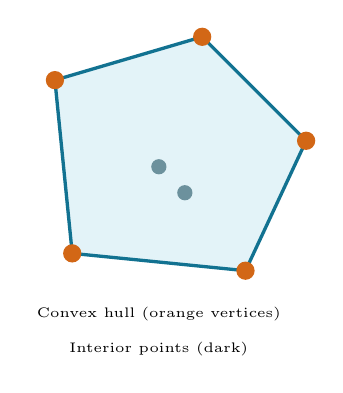
\begin{tikzpicture}[scale=1.1]
        \coordinate (A) at (0.5,0.5);
        \coordinate (B) at (2.5,0.3);
        \coordinate (C) at (3.2,1.8);
        \coordinate (D) at (2.0,3.0);
        \coordinate (E) at (0.3,2.5);
        \coordinate (F) at (1.5,1.5);
        \coordinate (G) at (1.8,1.2);
        \fill[PrimaryLight!40] (A)--(B)--(C)--(D)--(E)--cycle;
        \draw[PrimaryMid,very thick] (A)--(B)--(C)--(D)--(E)--cycle;
        \foreach \p in {A,B,C,D,E}{\fill[AccentOrange] (\p) circle(3pt);}
        \foreach \p in {F,G}{\fill[PrimaryDark!60] (\p) circle(2.5pt);}
        \node[font=\tiny] at (1.5,-0.2) {Convex hull (orange vertices)};
        \node[font=\tiny] at (1.5,-0.6) {Interior points (dark)};
      \end{tikzpicture}
      \newline
      \textbf{Complexity:} $\mathcal{O}(n^3)$
      (check all $O(n^2)$ edges, each with $O(n)$ point tests)
      
      More details \url{https://chebil.github.io/ConvexHull/}
      
  \end{columns}
\end{frame}

% ============================================================
\section{Exhaustive Search}
% ============================================================

\begin{frame}[shrink=12]{Exhaustive Search — What \& When}
  \begin{block}{Definition}
    \keyword{Exhaustive search} is a brute-force approach to combinatorial
    problems: generate \emph{all} candidate solutions, evaluate each,
    and keep the best.
  \end{block}
  \vspace{0.4em}
  \begin{columns}[T]
    \column{0.55\textwidth}
      \textbf{Typical structure:}
      \begin{enumerate}
        \item Generate all permutations / combinations / subsets
              of the input in a systematic way
        \item Evaluate each candidate solution
              (discard infeasible ones)
        \item Track the best feasible solution found so far
        \item When done, return the best
      \end{enumerate}
    \column{0.40\textwidth}
      \begin{alertblock}{When is it acceptable?}
        \begin{itemize}
          \item $n \leq 20$ for subset problems ($2^{20}\approx10^6$)
          \item $n \leq 12$ for permutation problems ($12!\approx5\times10^8$)
          \item When no efficient algorithm is known
          \item As a correctness baseline
        \end{itemize}
      \end{alertblock}
  \end{columns}
\end{frame}

\begin{frame}[shrink=12]{Travelling Salesman Problem (TSP)}
  \begin{columns}[T]
    \column{0.50\textwidth}
      \textbf{Problem:} Given $n$ cities and distances between every pair,
      find the \emph{shortest} tour that visits each city exactly once
      and returns to the start.

      \vspace{0.3em}
      \textbf{Brute-force:} Try all $(n-1)!/2$ distinct tours.

      \vspace{0.3em}
      \textbf{Example (4 cities):}
      \vspace{0.2em}

      \begin{tabular}{lr}
        \toprule
        \textbf{Tour} & \textbf{Cost} \\
        \midrule
        $a\to b\to c\to d\to a$ & $2+3+7+5=17$ \\
        $a\to b\to d\to c\to a$ & $2+4+7+8=21$ \\
        $a\to c\to b\to d\to a$ & $8+3+4+5=20$ \\
        $a\to c\to d\to b\to a$ & $8+7+4+2=21$ \\
        $a\to d\to b\to c\to a$ & $5+4+3+8=20$ \\
        $a\to d\to c\to b\to a$ & $5+7+3+2=\mathbf{17}$ \\
        \bottomrule
      \end{tabular}
    \column{0.45\textwidth}
      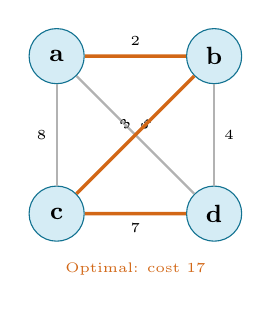
\begin{tikzpicture}[
        city/.style={circle,draw=PrimaryMid,fill=PrimaryLight!60,
                     font=\bfseries\small,minimum size=0.7cm},
        edge/.style={draw=gray!60,thick}
      ]
        \node[city] (a) at (0,2) {a};
        \node[city] (b) at (2,2) {b};
        \node[city] (c) at (0,0) {c};
        \node[city] (d) at (2,0) {d};
        \draw[edge] (a)--(b) node[midway,above,font=\tiny]{2};
        \draw[edge] (a)--(c) node[midway,left,font=\tiny]{8};
        \draw[edge] (a)--(d) node[midway,above,font=\tiny,sloped]{5};
        \draw[edge] (b)--(c) node[midway,above,font=\tiny,sloped]{3};
        \draw[edge] (b)--(d) node[midway,right,font=\tiny]{4};
        \draw[edge] (c)--(d) node[midway,below,font=\tiny]{7};
        \draw[AccentOrange,very thick,->]
          (a)--(b)--(c)--(d)--cycle;
        \node[font=\tiny,text=AccentOrange] at (1,-0.7)
          {Optimal: cost 17};
      \end{tikzpicture}
      \vspace{0.2em}
      \begin{alertblock}{Exponential growth}
        $\Theta(n!)$ — for $n=20$: $\approx 1.2\times10^{17}$ tours.
        At $10^9$ tours/sec: 4 million years.
      \end{alertblock}
  \end{columns}
\end{frame}

\begin{frame}[shrink=12]{0-1 Knapsack Problem}
  \begin{columns}[T]
    \column{0.55\textwidth}
      \textbf{Problem:} $n$ items with weights $w_i$ and values $v_i$;
      knapsack capacity $W$. Select a subset to maximise total value
      without exceeding capacity.

      \vspace{0.3em}
      \textbf{Brute force:} Examine all $2^n$ subsets.

      \vspace{0.3em}
      \textbf{Example} ($W=10$, 4 items):
      \vspace{0.2em}

      \begin{tabular}{lrr>{\small}l}
        \toprule
        \textbf{Subset} & \textbf{Weight} & \textbf{Value} & \\
        \midrule
        $\{1\}$       & 7 & 42 & \\
        $\{2\}$       & 3 & 12 & \\
        $\{3,4\}$     & 9 & \textbf{65} & \textcolor{SuccessGreen}{$\checkmark$ optimal} \\
        $\{1,2\}$     & 10 & 54 & \\
        $\{1,3\}$     & 11 & — & \alert{infeasible}\\
        \bottomrule
      \end{tabular}
    \column{0.40\textwidth}
      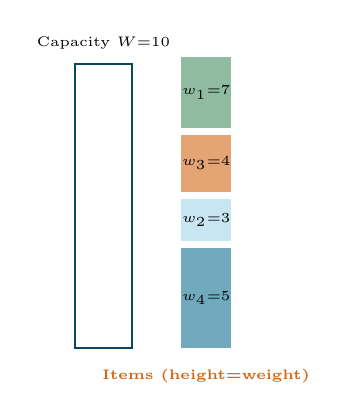
\begin{tikzpicture}[scale=0.9]
        \draw[PrimaryDark,thick] (0,0) rectangle (0.8,4);
        \node[font=\tiny] at (0.4,4.3) {Capacity $W$=10};
        % Items as colored blocks
        \fill[PrimaryMid!60] (1.5,0) rectangle (2.2,1.4);
        \fill[PrimaryLight!80] (1.5,1.5) rectangle (2.2,2.1);
        \fill[AccentOrange!60] (1.5,2.2) rectangle (2.2,3.0);
        \fill[SuccessGreen!50] (1.5,3.1) rectangle (2.2,4.1);
        \node[font=\tiny] at (1.85,0.7) {$w_4$=5};
        \node[font=\tiny] at (1.85,1.8) {$w_2$=3};
        \node[font=\tiny] at (1.85,2.6) {$w_3$=4};
        \node[font=\tiny] at (1.85,3.6) {$w_1$=7};
        \node[font=\tiny\bfseries,text=AccentOrange] at (1.85,-0.4)
          {Items (height=weight)};
      \end{tikzpicture}
      \vspace{0.2em}
      \begin{alertblock}{Complexity}
        \bigO{2^n} subsets to check.
        For $n=40$: $\approx 10^{12}$ subsets.
      \end{alertblock}
  \end{columns}
\end{frame}

\begin{frame}[shrink=12]{The Assignment Problem}
  \begin{columns}[T]
    \column{0.55\textwidth}
      \textbf{Problem:} Assign $n$ workers to $n$ jobs (one-to-one)
      to minimise total cost. Cost of worker $i$ doing job $j$ is $C[i,j]$.

      \vspace{0.3em}
      \textbf{Brute force:} Try all $n!$ permutations of jobs.

      \vspace{0.3em}
      \textbf{Example ($n=4$):}
      \vspace{0.2em}

      \begin{tabular}{*{5}{c}}
        \toprule
        & \textbf{Job 1} & \textbf{Job 2} & \textbf{Job 3} & \textbf{Job 4} \\
        \midrule
        P1 & 9 & 2 & 7 & 8 \\
        P2 & 6 & 4 & 3 & 7 \\
        P3 & 5 & 8 & 1 & 8 \\
        P4 & 7 & 6 & 9 & 4 \\
        \bottomrule
      \end{tabular}
      \vspace{0.2em}

      Assignment $\langle1,2,3,4\rangle$: $9+4+1+4 = \highlight{18}$ (optimal)
    \column{0.40\textwidth}
      \begin{alertblock}{Brute-force complexity}
        Must check all $n!$ permutations: for $n=20$ that is
        $\approx 2.4\times10^{18}$ assignments.
      \end{alertblock}
      \vspace{0.3em}
      \begin{exampleblock}{Better approach}
        The \emph{Hungarian Algorithm} solves the Assignment Problem
        in $\mathcal{O}(n^3)$ — we will revisit this in Ch.\ 5.
      \end{exampleblock}
      \vspace{0.3em}
      \textbf{This problem is NP-hard in general.}\\
      The assignment problem is solvable in polynomial time
      because of its special structure.
  \end{columns}
\end{frame}

% ============================================================
\section{BFS — Exhaustive Graph Search}
% ============================================================

\begin{frame}[shrink=12]{Shortest Path via Breadth-First Search}
  \begin{columns}[T]
    \column{0.50\textwidth}
      \begin{block}{BFS Algorithm}
        \begin{algorithmic}[1]
          \Require Graph $G$, source $s$, target $t$
          \State Enqueue $s$; $\text{parent}[s] \gets \text{null}$
          \While{queue not empty}
            \State $v \gets$ dequeue
            \If{$v = t$} \textbf{break} \EndIf
            \For{each neighbor $u$ of $v$}
              \If{$u \notin \text{parent}$}
                \State $\text{parent}[u] \gets v$
                \State enqueue $u$
              \EndIf
            \EndFor
          \EndWhile
          \State Trace back via \texttt{parent} to get path
        \end{algorithmic}
      \end{block}
    \column{0.45\textwidth}
      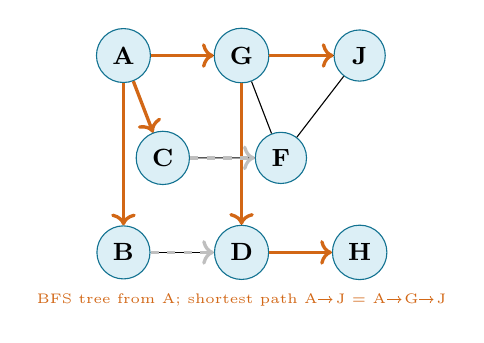
\begin{tikzpicture}[
        nd/.style={circle,draw=PrimaryMid,fill=PrimaryLight!50,
                   font=\bfseries\small,minimum size=0.65cm},
        vis/.style={circle,draw=AccentOrange,fill=AccentOrange!20,
                    font=\bfseries\small,minimum size=0.65cm},
        arr/.style={-{Stealth},PrimaryMid,thick}
      ]
        \node[nd] (A) at (0,2.5) {A};
        \node[nd] (G) at (1.5,2.5) {G};
        \node[nd] (J) at (3.0,2.5) {J};
        \node[nd] (C) at (0.5,1.2) {C};
        \node[nd] (F) at (2.0,1.2) {F};
        \node[nd] (B) at (0,0) {B};
        \node[nd] (D) at (1.5,0) {D};
        \node[nd] (H) at (3.0,0) {H};
        \draw (A)--(G)--(J); \draw (A)--(C)--(F)--(J);
        \draw (A)--(B)--(D)--(H);
        \draw (G)--(D); \draw (G)--(F);
        % BFS tree highlighted
        \draw[AccentOrange,very thick,->]
          (A)edge(G) (G)edge(J) (G)edge(D) (A)edge(C) (A)edge(B)
          (B)edge[dashed,gray!50](D) (D)edge(H) (C)edge[dashed,gray!50](F);
        \node[font=\tiny,text=AccentOrange] at (1.5,-0.6)
          {BFS tree from A; shortest path A→J = A→G→J};
      \end{tikzpicture}
  \end{columns}
  \vspace{0.3em}
  \begin{block}{Complexity}
    $\mathcal{O}(|V| + |E|)$ — visits every vertex and edge at most once.
    BFS guarantees \emph{shortest path} (minimum edges) in unweighted graphs.
  \end{block}
\end{frame}

% ── Chapter Summary ──────────────────────────────────────────
\begin{frame}[shrink=12]{Chapter 3 Summary}
  \begin{columns}[T]
    \column{0.52\textwidth}
      \textbf{Brute-force algorithms covered:}
      \begin{itemize}
        \item Selection sort, Bubble sort — $\Theta(n^2)$
        \item String matching — $\mathcal{O}(mn)$
        \item Closest pair — $\mathcal{O}(n^2)$
        \item Convex hull — $\mathcal{O}(n^3)$
      \end{itemize}
      \textbf{Exhaustive search:}
      \begin{itemize}
        \item TSP — $\Theta(n!)$
        \item 0-1 Knapsack — $\mathcal{O}(2^n)$
        \item Assignment — $\Theta(n!)$
        \item BFS shortest path — $\mathcal{O}(|V|+|E|)$
      \end{itemize}
    \column{0.44\textwidth}
      \begin{block}{Key insight}
        Brute force is a \emph{starting point}, not a destination.
        Understanding it clarifies what a better algorithm must
        improve upon.
      \end{block}
      \vspace{0.3em}
      \begin{block}{Next chapter}
        \textbf{Chapter 4:} Decrease \& Conquer + Divide \& Conquer —
        recursive strategies that break problems into smaller
        (or equal) sub-instances for dramatic efficiency gains.
      \end{block}
  \end{columns}
\end{frame}

\end{document}
